\documentclass[journal,twoside,web]{ieeecolor}

\makeatletter
\@ifpackageloaded{changes}{%
	\PackageWarning{}{changes already loaded, skipping}
	\let\usepackage\@gobble
}{}
\makeatother
\usepackage[markup=underlined,deletedmarkup=xout,authormarkup=brackets]{changes}





\usepackage[markup=underlined,deletedmarkup=xout,authormarkup=brackets]{changes}
%\definechangesauthor[name={Language Polish}, color=red]{}
% \usepackage{IEEE sensors journal}
\usepackage{jsen}
\usepackage{cite}
\usepackage{amsmath,amssymb,amsfonts}
\usepackage{algorithmic}
\usepackage{graphicx}
\usepackage{textcomp}
\usepackage{wrapfig}
\usepackage{multirow}
\usepackage{hyperref}
\hypersetup{
    colorlinks=true, 
    linkcolor=blue, 
    urlcolor=blue, 
    citecolor=blue, 
    pdfborder={0 0 0} 
}
\newtheorem{proposition}{Proposition}
\def\BibTeX{{\rm B\kern-.05em{\sc i\kern-.025em b}\kern-.08em
    T\kern-.1667em\lower.7ex\hbox{E}\kern-.125emX}}
\markboth{\journalname, VOL. XX, NO. XX, XXXX 2024}
{Author \MakeLowercase{\textit{et al.}}: Preparation of Papers for IEEE TRANSACTIONS and JOURNALS (May 2024)}
\definecolor{abstractbg}{rgb}{0.89804,0.94510,0.83137}
\setlength{\fboxrule}{0pt}
\setlength{\fboxsep}{0pt}

\begin{document}
\title{Dynamic Wi-Fi Fingerprinting in Contrastive Embedded Space for Robust Localization}
\author{F. Abbasi,  H. Sadoghi Yazdi
\thanks{ H. Sadoghi Yazdi and F. Abbasi are with the Department of Computer Engineering, Faculty of Engineering and the
Center of Excellence in Soft Computing and Intelligent Information Processing, Ferdowsi University of Mashhad, Mashhad, Iran (e-mail: h-sadoghi@um.ac.ir, abbasi.fa@mail.um.ac.ir). }}

\IEEEtitleabstractindextext{%
\fcolorbox{abstractbg}{abstractbg}{%
\begin{minipage}{\textwidth}%
\begin{wrapfigure}[12]{r}{3in}%
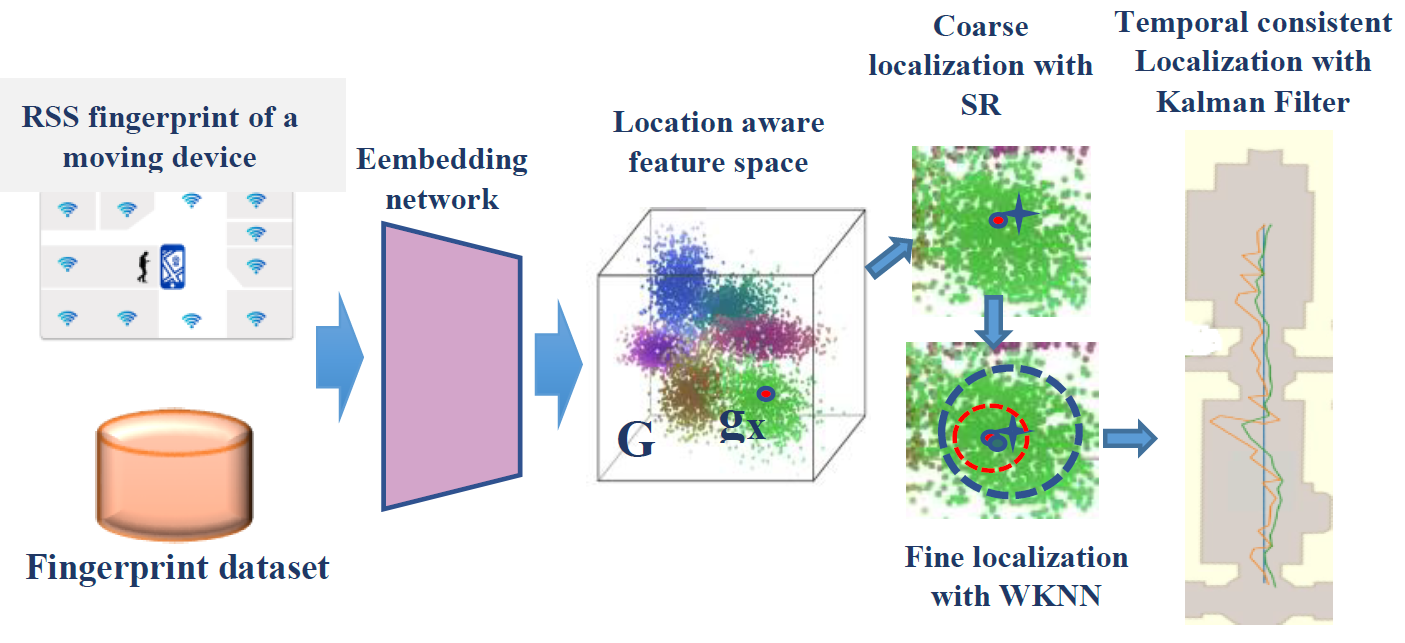
\includegraphics[width=3in]{pics2/abba1.png}%
\end{wrapfigure}%
\begin{abstract}
This paper presents a novel framework called CLIPS (Contrastive Learning Indoor Positioning System) for dynamic indoor positioning using Wi-Fi fingerprinting, which combines contrastive representation learning with sparse modeling and filtering methods.
In particular, we use contrastive representation learning to uncover the intrinsic spatial relationships between RSS signals.
% where nearby locations share similar representations while distant locations are well separated.
The method first computes an initial estimate of the location based on the Wi-Fi fingerprint embedding using sparse representation, and then refines the estimate through a local search.
In parallel, the Kalman filter handles motion dynamics efficiently, smoothing abrupt transitions and preserving the natural rhythm of spatial evolution over time. The integration of these methods results in more stable and generalizable location estimation. Experimental results show that the proposed method improves localization accuracy compared to traditional methods.
\end{abstract}
\begin{IEEEkeywords}
Wi-Fi Indoor Positioning, Contrastive Representation Learning, Kalman Filtering, Sparse Representation.
\end{IEEEkeywords}
\end{minipage}}}
\maketitle
\section{Introduction}
\label{sec:introduction}
\IEEEPARstart{I}{ndoor} positioning systems (IPS) are important in environments where GPS signals can be weak, such as large buildings and hospitals. Wi-Fi fingerprinting is one of the most common methods for indoor positioning.
Normally, Wi-Fi fingerprinting has two phases: in the offline phase, RSS readings at known positions are used to form a fingerprint database, and in the online phase, the current RSS profile is matched to estimate the location. Despite its popularity, Wi-Fi fingerprinting performance is often degraded by environmental conditions, multipath effects, and signal variability, which cause significant localization errors.

To align a new RSS profile with a fingerprinting dataset in the online phase, various methods have been proposed. Nearest-neighbor approaches remain among the most widely used due to their simplicity and effectiveness \cite{Bahl2000,RLWKNN,BMR_KNN}. Sparse representation methods have also been suggested \cite{SR2,STSR}, where a test fingerprint is expressed as a sparse linear combination of training samples.
More recent works extend to neural networks and deep learning \cite{Panja2024,Lan2022}. Metric learning methods such as triplet loss \cite{Triplet1,Triplet2} aim to learn embeddings where nearby fingerprints are close, and distant ones are well separated. To further enhance tracking performance, temporal models including RNNs \cite{RNN2}, LSTMs  \cite{LSTM1}, and filtering methods such as the Kalman filter have been employed \cite{PKF,EKF2,UKF2}.

While existing methods each leverage specific aspects of the latent information within RSS data, this approach intends  to  extract both spatial and temporal knowledge through a systematic, step-by-step process. CLIPS extracts the knowledge contained in RSS data by performing contrastive representation learning to inject spatial information into the feature space, followed by sparse modeling for progressive extraction of this knowledge, and dynamic filtering with the Kalman filter to encode temporal knowledge of feature evolution. Our work makes several contributions:
\begin{enumerate}
    \item  
    Using contrastive metric learning (specifically, InfoNCE loss), spatial knowledge within RSS data is extracted. Training the model to separate nearby from distant signal patterns, improves sensitivity to subtle spatial variations and enhances localization accuracy.
    \item 
    A hierarchical matching strategy is employed: coarse localization via sparse representation, followed by refinement within the local neighborhood. This stepwise approach takes advantage of spatial continuity in Wi-Fi signals for a more robust position estimation.  
    \item  
    A Kalman filter is used to smooth abrupt variations and track temporal evolution. This improves stability and reliability in dynamic indoor environments. 
    \item 
    Extensive experiments have been  performed on a real-world dataset collected from our academic building and benchmark datasets.
\end{enumerate}
In the following sections, Section II reviews related work. Section III presents the proposed method. Section IV reports experimental evaluations, and Section V is the conclusion of this article.
\section{Related Works}
The idea of fingerprinting was first introduced by Bahl and Padmanabhan in the RADAR study \cite{Bahl2000}, where it was described that it is possible to estimate the device location based on RSS readings at different locations and then to match the received signal pattern with the known reference stored in the database. This work was pioneering in applying the k-nearest neighbors (KNN) algorithm for fingerprint matching.

KNN and its variants are widely used for fingerprint matching due to their simplicity and effectiveness. Weighted KNN (WKNN) improves performance by assigning higher weights to closer neighbors. Various studies have focused on enhancing WKNN through adaptive selection of $k$ \cite{BMR_KNN}, alternative distance metrics \cite{ RLWKNN}, and improved weighting schemes \cite{WKNNW}.

Another approach that has been proposed for fingerprint matching is sparse representation (SR).
SR models a test fingerprint as a sparse linear combination of training samples, assuming that spatially close points share similar RSS patterns. However, this assumption may not always hold due to complex indoor signal propagation, where RSS similarity does not necessarily imply physical proximity \cite{WKNN7, ref1}. Despite this limitation, SR has been successfully applied in indoor localization \cite{STSR, SR2}.

For large datasets, the comparison of an online fingerprint with the full database directly is computationally expensive. To address this, hierarchical techniques divide localization into two steps. (1) Coarse localization, which estimates the general location of the device. Some common approaches in this setp are RSS clustering \cite{clustering} and coordinate clustering \cite{Two_step_localization1}. 
(2) Fine localization where methods such as WKNN or Sparse Representation \cite{SR2} are used to refine the estimate.
This two-step strategy improves computational performance by reducing candidate locations before the final accurate estimation. It is especially important in dynamic environments where real-time tracking is required.

In recent years, deep neural networks (DNNs) \cite{Lan2022} and autoencoders (AEs) \cite{Panja2024} have become important methods for deriving informative features from raw RSS data. While these methods preserve RSS distribution, they may fail to maintain spatial continuity of RSS fingerprints.
To solve this problem, metric learning approaches aim to learn an embedding space where RSS fingerprints from nearby locations are mapped closer together.
In \cite{Triplet1} and \cite{Triplet2} Siamese networks with triplet loss have been used for this purpose.
However, triplet loss suffers from challenges such as sensitivity to triplet selection and its focus on local relationships within triplets.
Another popular contrastive loss function is InfoNCE. InfoNCE uses multiple negative samples per anchor and avoids complex sample selection. This leads to more discriminative embeddings with improved efficiency and generalization.

All of the above-mentioned methods are kinds of static localization. 
In contrast, dynamic localization continuously estimates the position of a moving object by considering temporal dependencies between consecutive RSS measurements.
Recurrent models \cite{RNN2, LSTM1} and filtering techniques such as Kalman and particle filters \cite{PKF, FKF, EKF2, UKF2} are well suited for processing such sequential data. Kalman filter combines motion models with sensor data to improve accuracy, reduce noise, and ensure continuity over time. The position Kalman filter (PKF) \cite{PKF} uses static position solutions as measurements, while the fingerprint Kalman filter (FKF) \cite{FKF} works directly with the measured signal strength. Variants like extended Kalman filter (EKF) \cite{EKF2} and unscented
Kalman filter (UKF) \cite{UKF2} have also demonstrated strong performance.

The goal of this paper is to gradually extract spatiotemporal knowledge within RSS data.
Contrastive metric learning is used to map RSS vectors into a feature space where physical location information is preserved. For the first time, the method explores the capabilities of the InfoNCE loss function for indoor localization.
To extract the latent knowledge from the learned space, a coarse-to-fine localization process is employed. Unlike other methods that have used Sparse Representation for precise localization, this paper employs it for coarse localization. As a result, while benefiting from the advantages of SR in location estimation, it remains less vulnerable to its inaccuracies. Finally, Kalman filtering is used to extract the temporal knowledge presented in sequential data according to a physical motion model.
\section{Proposed Method}
The CLIPS formulation is defined as follows.
 Let \(\mathbf{D_{train}} = [ F,C], \quad \mathbf F \in \mathbb{R}^{N\times M}, \quad \mathbf C \in \mathbb{R}^{N\times d}\), be the training dataset consisting of fingerprint data of each reference point (RP) and their corresponding coordinates.     
 Where $N$ is the number of RPs in the database, $M$ is the number of Wi-Fi access points (APs), and $d$ is the dimensionality of the location space, which in our case is 2D.
$\mathbf{F}=[\mathbf{f}_i]_{i=1}^N$ is a fingerprint matrix, whose rows consist of RSS values from multiple APs at known RP's location (\(    \mathbf{f}_{i} = [RSS_{ij}]_{j=1}^M\)) and $\mathbf{C}=[\mathbf{c}_i]_{i=1}^N$ is the corresponding set of coordinates for the fingerprints
(\(\mathbf{c}_{i} = [latitude_i,longitude_i] \)).

Let $x$ be a test sample and $\mathbf{f}_{x}= [RSS_1, RSS_2, ..., RSS_M] \in \mathbb{R}^{M}$ be the observed RSS vector for this new sample with an unknown location.
The goal is to estimate the location $\mathbf{\hat{c}_x}$ corresponding to $\mathbf{f}_{x}$.
\subsection{Overview}
The proposed CLIPS consists of two
phases:

1) Offline phase: 
\begin{itemize}
    \item After collecting and preprocessing RSS data, Wi-Fi fingerprints  
    \(\mathbf{F}\)  
    and their corresponding locations 
    \(\mathbf{C} \), are stored in fingerprint database.
    \item The next step is to learn an embedding function \( g: \mathbb{R}^M \to \mathbb{R}^D \) that utilizes contrastive learning to incorporate spatial information into the embedding space.
\end{itemize}
2) Online phase:
\begin{itemize}
    \item In the static localization stage, the static location at time \( t \), denoted as \( \tilde{c}_{x_t} \), is estimated for an input RSS vector embedding \( g(f_{x_t}) \) using sparse representation and WKNN in a two-step coarse-to-fine localization process.
    \item In the dynamic localization stage, the noisy estimates from the static localization phase are processed by a Kalman filter to obtain smooth and spatiotemporally consistent position estimates, denoted as \( \hat{c}_{x_t} \).
\end{itemize}
Fig.~\ref{proposed_method3} dets the
two phases and the main steps of CLIPS. In the following subsections, the offline phase (Learning a New Space) and the online phase (static localization –Fig.~\ref{proposed_method3} steps 1–6; dynamic localization – Fig.~\ref{proposed_method3} step 7) are described in detail.
\begin{figure*}[!t]
\centerline{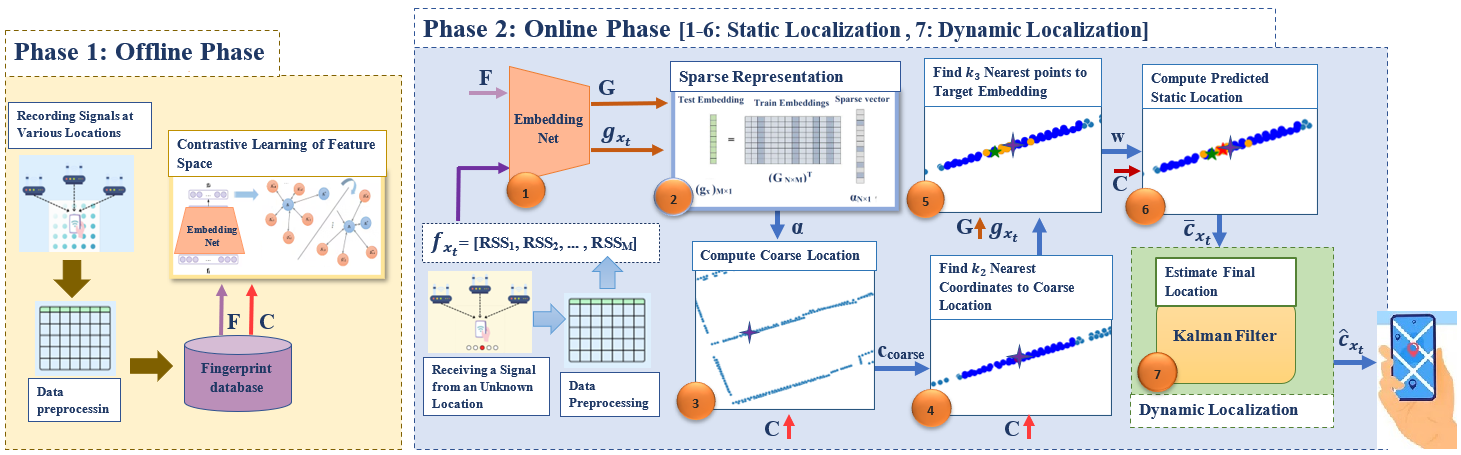
\includegraphics[width=\textwidth]{pics2/abba2.png}}
\caption{An overview of the CLIPS. In the offline phase, RSS values from M  Access Points are collected and preprocessed to construct fingerprint map (F are fingerprints and C are coordinates]. Subsequently, a neural network is trained with a contrastive loss function to project the fingerprints into a latent space where spatial proximity corresponds to similarity in representation.
In the online phase, at step (1), fingerprints from train and test data (F,$f_x$) are mapped to the feature space (G, $g_x$). In step (2) sparse representation estimates the coefficient vector \(\alpha\). In step (3), the coarse location is estimated by averaging the coordinates of the data points with the highest coefficients. In step (4), the \(k_2\) nearest points to the coarse location in the coordinate space are selected, and from them, in step (5) the \(k_3\) closest points in the embedding space (yellow) are chosen. In step (6), the static location, $\tilde c_x$ (red star) is computed as a weighted average of these \(k_3\) points. The green star represents the true location, $c_x$. Finally, In step (7), dynamic location ($\hat c_{x_t}$) is obtained through Kalman filtering.}
\label{proposed_method3}
\end{figure*}
\subsection{Offline Phase: Learning a New Space}
After site survey and preprocessing of fingerprint data in the offline phase, contrastive metric learning is employed. 
Given the set of Wi-Fi fingerprints
\(\mathbf{F} = \{ \mathbf{f}_i \}_{i=1}^{N}\) 
and their corresponding locations
\(\mathbf{C} = \{ \mathbf{c}_i \}_{i=1}^{N} \), 
our goal is to learn an embedding function
\( g : \mathbb{R}^M \to \mathbb{R}^D \) 
that maps each fingerprint \(\mathbf{f}_i\) 
to a lower-dimensional feature space, ensuring that fingerprints from nearby locations remain close while those from distant locations are pushed apart.
A neural network \( g \) is defined to transform a fingerprint \( \mathbf{f}_i \) into an embedding $g(\mathbf{f}_i) \in \mathbb{R}^D$. Two commonly used contrastive loss functions for network training are triplet loss and InfoNCE loss.
\subsubsection{Triplet Loss}
 Triplet loss ensures that an anchor sample embedding \( \mathbf{g}(\mathbf{f_i}) \) is closer to a positive sample embedding \( \mathbf{g(f_i^+)} \) from the same location than to a negative one  \( \mathbf{g(f_i^-)} \) from a different location. For simplicity, in the rest of the paper \( \mathbf{g_i} \) is used instead of \( \mathbf{g(f_i)} \) to represent the transformed fingerprint \( \mathbf{f_i} \) in the embedding space. 
 \begin{equation}
L_{Triplet} = \frac{1}{N} \sum_{i=1}^{N} \max(\| g_i - g_i^+) \|_2^2 - \| g_i - g_i^-) \|_2^2 + m, 0) .
\end{equation}
where $m$ is the margin that enforces a minimum separation between positive and negative pairs.
\subsubsection{InfoNCE Loss}
 InfoNCE enhances similarity learning by maximizing agreement between similar pairs while minimizing agreement with negative examples. Each fingerprint \( \mathbf{f}_i \) (anchor) is associated with a positive fingerprint \( \mathbf{f}_i^+ \) (from a nearby location) and a set of multiple negative fingerprints 
\( \mathcal{N}_i=\{\mathbf{f}_{i,k}^-\}_{k=1}^{ |\mathcal{N}_i|} \), (from distant locations). 
The InfoNCE loss is defined as:
\begin{equation}
\tiny
L_{\text{InfoNCE}} = -\frac{1}{N} \sum_{i=1}^{N} \log \left(
\frac{
\exp\left( \frac{\text{sim}(g_i, g_i^+)}{\tau} \right)
}{
\exp\left( \frac{\text{sim}(g_i, g_i^+)}{\tau} \right)
+  \sum_{k=1}^{|\mathcal{N}_i|} \exp\left( \frac{\text{sim}(g_i, g_{i,k}^-)}{\tau} \right)
}  \right).
\label{eq:infonce-loss}
\end{equation}
where \( \tau \) is a temperature scaling parameter, \( sim(.) \) is the similarity between the anchor and its positive sample and is usually measured using the cosine similarity:
\begin{equation}
 sim(g_i,g_j) = \frac{g_i^\top g_j}{\|g_i\| \|g_j\| }.
\end{equation}
The denominator of the InfoNCE loss equation ensures that positive pairs are assigned higher probabilities.
\subsubsection{Positive and negative selection} 
In our custom dataset, positives and negatives were selected offline from the entire dataset before training the network and for benchmark datasets samples are selected online at each epoch.

In custom dataset, Under both loss function setups, for each anchor, a predefined number of positive samples are chosen as the nearest neighbors in the coordinate space, and for each of them, negatives are randomly selected from other fingerprints.
In benchmark datasets, For each anchor, a fixed number of positive samples are chosen as the nearest neighbors within a predefined coordinate distance threshold. Negative samples are randomly drawn from the remaining samples outside this threshold for each anchor-positive pair.
\subsection{Online Phase: Static Localization (Steps 1–6)}
In this stage, 
first, the test RSS vector is mapped into the learned feature space. Subsequently, the test features are represented as a sparse linear combination of training features by solving a sparse representation problem, from which a coarse location estimate is obtained. Finally, WKNN is applied to the nearby points of coarse location to refine the position estimate.
\subsubsection{Coarse Localization with Sparse Representation}
Once the test embedding is obtained, sparse representation is used to find an approximate location for the test sample. Sparse representation is a mathematical technique that models a signal as a linear combination of small number of samples selected from a dictionary. Given a set of training data embeddings \(  \mathbf{G} = \{ \mathbf{g}_1, \mathbf{g}_2, \dots, \mathbf{g}_N \} \) as the dictionary and corresponding location coordinates \( \mathbf{C} = \{ \mathbf{c}_1, \mathbf{c}_2, \dots, \mathbf{c}_N \} \),  the goal is to estimate the approximate location \( \mathbf{c}_{coarse} \) of a test embedding \( \mathbf{g}_x \). The idea is to express a test embedding $ \mathbf{g}_x $ as a sparse linear combination of training embeddings:
\begin{equation}
    g_x \approx \sum_{i=1}^{N} \alpha_i g_i .
\end{equation}
where \( \alpha \) is a non-negative sparse coefficient vector that determines the contribution of each training point. The sparse representation problem is formulated as:
\begin{equation}
    \min_{\alpha} \lambda \| \alpha \|_1 + \frac{1}{2}\left\| g_x - G^T \alpha \right\|_2^2 .
\end{equation}
where \( \mathbf{\lambda} \) is a regularization parameter controlling sparsity (in our experiments, \( \mathbf{\lambda}=0.5 \)).
After solving for \( \mathbf{\alpha} \), The top \( k_1 \) training points with the largest coefficients \( \mathbf{\alpha}_i \) are selected. The estimated coarse location is computed as a weighted average:
\begin{equation}
    c_{coarse} = \frac{\sum_{i \in S} \alpha_i c_i}{\sum_{i \in S} \alpha_i}.
\end{equation}
where \( S \) is the set of top \( k_1 \) indices.
\subsubsection{Fine Localization with WKNN}
In this step the estimated coarse position is refined using a nearest neighbor selection process. 
First, the Euclidean distance between the coarse location $\mathbf{c}_{\text{coarse}}$ and each training coordinate $\mathbf{c}_i$ is computed as:
\begin{equation}
    d_i = \| \mathbf{c}_{\text{coarse}} - \mathbf{c}_i \|_2 .
\end{equation}
The $k_2$ nearest neighbors with the smallest $d_i$ values are selected as the set $U$.
 For each of the $k_2$ selected neighbors, their Euclidean distance with the test sample in the embedding space is computed:
\begin{equation}
    d_j' = \| g_{\text{x}} - g_j \|_2 , \quad j \in U .
\end{equation}
where $g_{\text{x}}$ is the embedding of the test point, and $g_j$ is the embedding of each selected neighbor. Then, $k_3 < k_2$ closest points in embedding space are chosen to form the set $L$.
The final estimated location is computed as a weighted average.
\begin{equation}
    \mathbf{\tilde{c}}_{\text{x}} = \frac{\sum_{l \in L } w_l \mathbf{c}_l}{\sum_{l \in L} w_l}, \quad  w_l = \frac{1}{d_l' + \epsilon }.
\end{equation}
 where $\epsilon$ is a small constant to prevent division by zero. 
\subsection{Online Phase: Dynamic Localization (Step 7)} 
The dynamic nature of indoor spaces, characterized by moving obstacles and changing device configurations, necessitates a more adaptable approach to maintain localization accuracy over time.
The proposed method applies a Kalman filter in a guided feature space to address this situation. Kalman filter is an optimal recursive algorithm used for estimating the state of a dynamic system in the presence of noise. The proposed method uses a  Kalman filter with a Constant Acceleration state-space model as follows: 
\subsubsection{State-Space Model} 
The state \( \mathbf{s}_t \) at time \( t \) is defined as:
\begin{equation}
\scalebox{0.85}{$
 \mathbf{s}_t = \begin{bmatrix} lat_t & lon_t & v\_lat_t & v\_lon_t & a\_lat_t & a\_lon_t \end{bmatrix}^T . $}
\end{equation}
where \(lat_t\) and  \(lon_t\) are the device’s position at time \(t\), \(v\_lat_t\) and  \(v\_lon_t\) are the corresponding velocity components and \(a\_lat_t\) and \(a\_lon_t\) represent acceleration. 
The state evolution follows a Constant Acceleration model:
\begin{equation}
\mathbf{s}_{t+1} = A\mathbf{s}_t + \mathbf{w}_t, \quad \mathbf{w}_t \sim \mathcal{N}(0, \mathbf{Q}).
\end{equation}
where \( \mathbf{w}_t \) is process noise with covariance \( \mathbf{Q} \) and \(A\) is state transition model.
\begin{equation}
\scalebox{0.85}{$
    \mathbf{A} = \begin{bmatrix}  
        1 & 0 & \Delta t & 0 & \frac{\Delta t^2}{2}  & 0\\
        0 & 1 & 0 & \Delta t & 0 & \frac{\Delta t^2}{2}\\
        0 & 0 & 1 & 0 & \Delta t & 0\\
        0 & 0 & 0 & 1 & 0 &  \Delta t \\
        0 & 0 & 0 & 0 & 1 & 0 \\
        0 & 0 & 0 & 0 & 0 & 1 \\
    \end{bmatrix}, \quad $}   
\end{equation} 
\subsubsection{Observation Model}
The observation \( \mathbf{z}_t \) corresponds to the static estimate \( \tilde c_{x_t} \) and the observation model is defined as:
\begin{equation}
\scalebox{0.85}{$
\mathbf{z}_t = H\mathbf{s}_t + \mathbf{v}_t, \quad \mathbf{v}_t \sim \mathcal{N}(0, \mathbf{R}), \quad 
 H = \begin{bmatrix}
    1 & 0 & 0 & 0 & 0 & 0\\
    0 & 1 & 0 & 0 & 0 & 0\\
\end{bmatrix} $}
\end{equation}
where \( \mathbf{v}_t \) is observation noise with covariance \( \mathbf{R} \) and \(H\) is the observation matrix.
\subsubsection{Kalman Filter Equations}
The Kalman filter consists of two steps, (1) the prediction step, in which the predicted state $\hat{\mathbf{s}}_{t|t-1}$ and predicted covariance matrix $\mathbf{P}_{t|t-1}$ are computed as:
\begin{equation}
\small
 \hat{\mathbf{s}}_{t|t-1} = A\hat{\mathbf{s}}_{t-1|t-1},
\end{equation}
\begin{equation}
\small
\mathbf{P}_{t|t-1} = A\mathbf{P}_{t-1|t-1}A^T + \mathbf{Q}.
\end{equation}
and (2) the update step, where the Kalman gain \(\mathbf{K}_t\) is computed, and the final estimated state \(\hat{\mathbf{s}}_{t|t}\) is obtained using the observation \(\mathbf{z}_t\):
\begin{equation}
\small
\mathbf{K}_t = \mathbf{P}_{t|t-1} H^T (H\mathbf{P}_{t|t-1} H^T + \mathbf{R})^{-1},
\end{equation}
\begin{equation}
\hat{\mathbf{s}}_{t|t} = \hat{\mathbf{s}}_{t|t-1} + \mathbf{K}_t (\mathbf{z}_t - H\hat{\mathbf{s}}_{t|t-1}),
\end{equation}
\begin{equation}
\small
\mathbf{P}_{t|t} = (\mathbf{I} - \mathbf{K}_t H) \mathbf{P}_{t|t-1}.
\end{equation} 
For each test sample \( x_t \) in a trajectory, the final position estimate is:
\begin{equation} 
\mathbf{\hat c}_{x_t} =H \hat{\mathbf{s}}_{t|t} .\end{equation}  
It can be proven that, under certain assumptions, the Kalman filter's dynamic estimate always provides a more accurate estimate than the static one, as it refines the prediction over time by incorporating new measurements and system dynamics.
\begin{proposition}[Optimal Refinement]  
		The Kalman-filtered estimate $\hat{\mathbf{c}}_{x_t}$ satisfies:  
		\begin{equation}
		\mathbb{E}\left[ \| \mathbf{c}_{x_t} - \hat{\mathbf{c}}_{x_t} \|_2^2 \right] \leq \mathbb{E}\left[ \| \mathbf{c}_{x_t} - \tilde{\mathbf{c}}_{x_t} \|_2^2 \right].
		\end{equation}   
\end{proposition}  
where \(\mathbf{c}_{x_t}\) is the ground truth position of $x_t$ and \(\tilde{\mathbf{c}}_{x_t}\) and \(\hat{\mathbf{c}}_{x_t}\) are static and dynamic position estimates respectively (to see the proof, please refer to Appendix A).
\subsection{Computational Analysis}
The computational complexity of the offline phase is not critical as it is performed only once. In the online phase, which is critical for real-time localization, the complexity is mainly dominated by the sparse representation step, scaling as \(O(TND)\)  using CVXPY solver, where \(T\) is the solver iteration count.
Feature embedding is efficient, with a cost of 
\(O(MH + LH^2)\) per fingerprint, where \(L\) is number of network layers and \(H\) is the average layer size. Fine localization via WKNN involves \(O(N + k_2 D)\) for neighbor selection and distance computation, while dynamic refinement using Kalman filtering has constant complexity \(O(1)\)
per update.
\section{EXPERIMENTS}
\subsection{Experimental Data}
\subsubsection{Custom Dataset}
Wi-Fi fingerprint data was collected from the Faculty of Engineering, Ferdowsi University of Mashhad, Iran (36.3105° N, 59.5299° E) and includes multiple floors with undetected access points marked as -100 dBm. Each sample consists of RSS values from 81 APs, geographical coordinates, and floor level (floor 2 used here). Fig.~\ref{fig:static_dynamic_train_test} illustrates the Faculty of Engineering and the static/dynamic training (green) and testing (blue) points. Dataset details are summarized in Table~\ref{tab:Dtatsets}.
\begin{figure}[t]
\centering
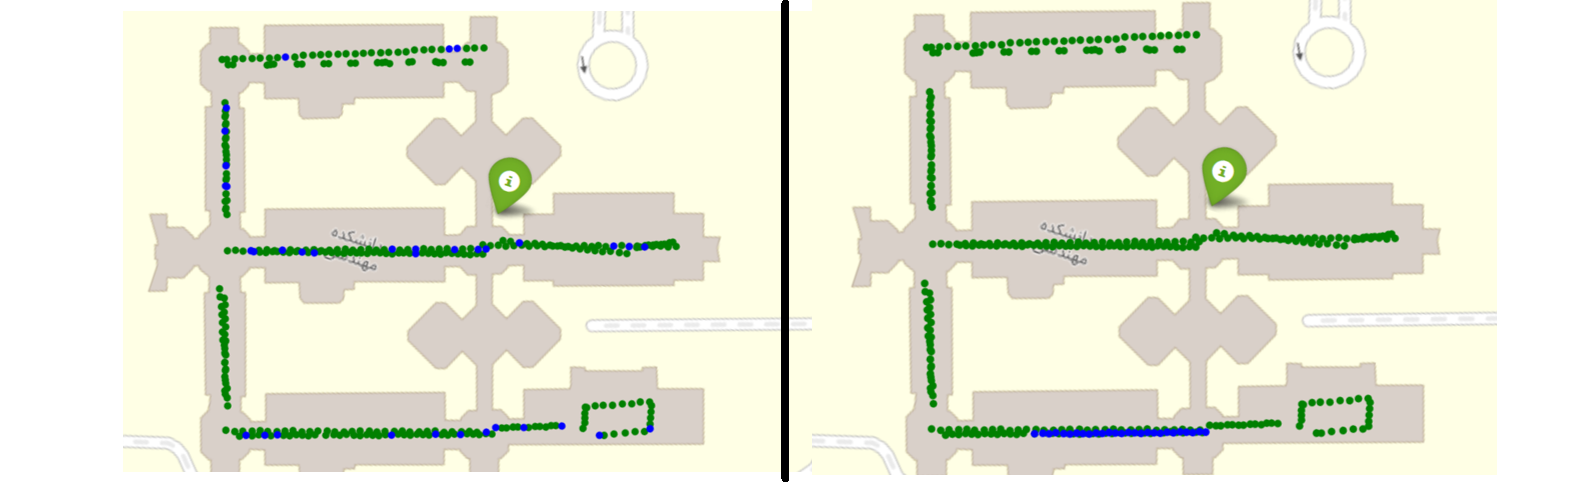
\includegraphics[width=\columnwidth]{pics2/abba3.png}
\caption{Static (left) and dynamic (right) training (green) and testing (blue) data.}
\label{fig:static_dynamic_train_test}
\end{figure}
\begin{table}[!t]
\centering
\caption{Overview of the Experimental Datasets}
\label{tab:Dtatsets}
\resizebox{\columnwidth}{!}{%
\begin{tabular}{lcc}
\hline
\textbf{Dataset} & \textbf{Samples} & \textbf{Features (WAPs)} \\ \hline
Static Custom Dataset & 349 (314 train / 35 test) & 81 WAPs \\ 
Dynamic Custom Dataset & 375 (348 train / 27 test) & 81 WAPs \\
UJIIndoorLoc & 5,984 (5,636 train / 348 test) & 520 WAPs \\
Geotec & 1,140 (680 train / 460 test) & 97 WAPs  \\ \hline
\end{tabular} %
}
\end{table}
\subsubsection{Benchmark Datasets}
We additionally evaluate the proposed method on two benchmark datasets: UJIIndoorLoc \cite{refUJIIndoorLoc} and Geotec \cite{refGeoTech}. Key dataset statistics are summarized in Table~\ref{tab:Dtatsets}. Since UJIIndoorLoc is a multi-building and multi-floor dataset, we select the floor with the most training samples per building for 2D localization. 
\subsection{Experimental Setup}
The experiments are divided into two parts, static and dynamic localization experiments. For static localization, the performance is evaluated by various metrics including mean localization error (MLE), mean absolute error (MAE), root mean square error (RMSE), and percentile errors across different embedding spaces. Statistical significance is also illustrated using the cumulative distribution function (CDF). In addition, we report the average processing time per fingerprint in the online phase as a measure of the computational efficiency. 
For dynamic localization, we report the MLE of different motion models. All tests were conducted on a 64-bit Windows 10 Pro, with an Intel Core i7 processor (\(\sim 4.2\) GHz), 16~GB of RAM, and Python 3.9. 
Method parameters were obtained using a sequential coarse-to-fine grid search, and their values are reported in Table \ref{tab:method parameters}. 
\subsubsection{Embedding Network Structure and Training Setup}
For all models a fully connected neural network with two hidden layers and a 32-dimensional output layer using ReLU activations and Batch Normalization was adopted. For benchmark datasets dropout (rate = 0.1) and L2 normalization (on the output layer) were additionally used. All models were trained using Adam optimizer (learning rate 0.001, batch size 256).

Table~\ref{tab:training-setup} provides details of training configurations adopted for the neural network models across the evaluated datasets.
\begin{table*}[!t]
\centering
\caption{Parameter Setup for SR + WKNN Method}
\label{tab:method parameters}
% \tiny
\resizebox{\textwidth}{!}{%
\begin{tabular}{l|c|c|c||c|c|c||c|c|c}
\hline
\multirow{2}{*}{\textbf{Parameters}} 
& \multicolumn{3}{c||}{\textbf{Custom Dataset}} 
& \multicolumn{3}{c||}{\textbf{UJIIndoorLoc Dataset}} 
& \multicolumn{3}{c}{\textbf{Geotec Dataset}} \\ \cline{2-10}
& \textbf{RSS} & \textbf{Triplet} & \textbf{InfoNCE} 
& \textbf{RSS} & \textbf{Triplet} & \textbf{InfoNCE} 
& \textbf{RSS} & \textbf{Triplet} & \textbf{InfoNCE } \\ \hline
 (k1, k2, k3) & (5, 41, 3)   & (2, 36, 7) & (6, 35, 3) & --- & (40, 355, 22) & (10, 70, 15) & (20, 250, 9) & (8, 300, 10) & (20, 165, 11)  \\ \hline
\end{tabular} %
}
\end{table*}
\begin{table*}[!t]
\centering
\caption{Training Setup for Triplet Loss and InfoNCE Loss Models Across Datasets}
\label{tab:training-setup}
\tiny
\resizebox{\textwidth}{!}{%
\begin{tabular}{l|c|c||c|c||c|c}
\hline
\multirow{2}{*}{\textbf{Configuration}} 
& \multicolumn{2}{c||}{\textbf{Custom Dataset}} 
& \multicolumn{2}{c||}{\textbf{UJIIndoorLoc Dataset}} 
& \multicolumn{2}{c}{\textbf{Geotec Dataset}} \\ \cline{2-7}
& \textbf{Triplet Loss} & \textbf{InfoNCE Loss} 
& \textbf{Triplet Loss} & \textbf{InfoNCE Loss} 
& \textbf{Triplet Loss} & \textbf{InfoNCE Loss} \\ \hline
Hidden Layers   & [128, 64] & [128, 64] & [512, 128] & [512, 128] & [128, 64] & [128, 64] \\ \hline
Training Epochs & 3 & 5 & 4 & 4 & 10 & 14 \\ \hline
Loss Parameter  & Margin=0.3 & Temperature=0.7 & Margin=0.7 & Temperature=0.1 & Margin=0.7 & Temperature=0.7 \\ \hline
\end{tabular} %
}
\end{table*}
\begin{table*}[t]
\centering
\caption{Error Metrics (in Meters), Percentile Localization Errors (P50/P75/P90), and Computation Time (Average per Test Sample in ms) for Various Static Methods in Different Feature Spaces on Custom Dataset}
\resizebox{\textwidth}{!}{%
\begin{tabular}{c|ccccccc|ccccccc|ccccccc}
\hline
\multirow{2}{*}{\textbf{Method}} & \multicolumn{7}{c|}{\textbf{RSS Space}} & \multicolumn{7}{c|}{\textbf{Triplet Space}} & \multicolumn{7}{c}{\textbf{InfoNCE Space }} \\
 & MLE & RMSE & MAE & P50 & P75 & P90 & Time & MLE & RMSE & MAE & P50 & P75 & P90 & Time & MLE & RMSE & MAE & P50 & P75 & P90 & Time \\
\hline
WKNN & 6.63 & 8.73 & 4.17 & 5.02 & 8.85 & 16.15 & \textbf{0.22} & 7.30 & 9.77 & 4.63 & 5.09 & 8.26 & 15.62 & \textbf{0.11} & 7.41 & 11.41 & 4.76 & 4.96 & 8.69 & 15.06 & \textbf{0.11} \\
K-Means + WKNN & 6.85 & 10.56 & 4.36 & 4.93 & 8.24 & 13.81 & 0.95 & 6.13 & 8.33 & 3.86 & 4.36 & 7.37 & 12.36 & 0.86 & 9.67 & 16.51 & 6.34 & 5.07 & 11.42 & 17.91 & 1.00 \\
SR & 9.46 & 12.22 & 6.03 & 8.19 & 15.40 & 21.38 & 77 & 8.50 & 11.25 & 5.45 & 6.22 & 12.25 & 17.49 & 37 & 8.62 & 12.18 & 5.59 & 6.11 & 9.81 & 17.22 & 38 \\
SR + SR & 8.12 & 10.66 & 5.18 & \textbf{4.72} & 11.41 & 16.76 & 96 & 7.03 & 8.72 & 4.47 & \textbf{4.15} & 11.06 & 13.17 & 55 & 6.90 & 8.67 & 4.40 & 4.75 & 9.47 & 14.18 & 56 \\
SR + WKNN  & \textbf{5.54} & \textbf{7.30} & \textbf{3.47} & 4.90 & \textbf{7.36} & \textbf{12.47} & 74 &  \textbf{5.42} & \textbf{6.73} & \textbf{3.42} & 4.19 & \textbf{7.23} & \textbf{10.42} & 37 &  \textbf{5.12} & \textbf{6.63} & \textbf{3.21} & \textbf{3.68} & \textbf{7.16} & \textbf{11.32} & 38 \\
\hline
\end{tabular}%
}
\label{tab:static_errors}
\end{table*}
\begin{table*}[t]
\centering
\caption{Mean Localization Error (in Meters) and Computation Time (Average per Test Sample in ms) on UJIIndoorLoc and Geotec Datasets}
% \scriptsize
\tiny
\resizebox{\textwidth}{!}{%
\begin{tabular}{c|cc|cc|cc||cc|cc|cc}
\hline
\multirow{3}{*}{\textbf{Method}} 
& \multicolumn{6}{c||}{\textbf{UJIIndoorLoc Dataset}} 
& \multicolumn{6}{c}{\textbf{Geotec Dataset}} \\
\cline{2-13}
& \multicolumn{2}{c|}{\textbf{RSS Space}} 
& \multicolumn{2}{c|}{\textbf{Triplet Space}} 
& \multicolumn{2}{c||}{\textbf{InfoNCE Space}} 
& \multicolumn{2}{c|}{\textbf{RSS Space}} 
& \multicolumn{2}{c|}{\textbf{Triplet Space}} 
& \multicolumn{2}{c}{\textbf{InfoNCE Space}} \\
\cline{2-13}
 & MLE & Time & MLE & Time & MLE & Time & MLE & Time & MLE & Time & MLE & Time \\
\hline
WKNN            & 10.09 & 18.12 & \textbf{8.74} & \textbf{0.64} & \textbf{7.60} & \textbf{0.66} & 4.28 & \textbf{0.32} & \textbf{3.81} & \textbf{0.20} & \textbf{3.86} &\textbf{0.23} \\
K-Means + WKNN  & \textbf{9.32} & \textbf{15.05} & 8.81 & 2.40 & 7.65 & 2.43 & 4.40 & 1.26 & 3.83 & 1.15 & 3.94 & 1.18 \\
SR              & -- & -- & 9.25 & 838 & 8.39 & 903 & 4.33 & 182.99 & 3.89 & 61.19 & 3.93 & 63.05 \\
SR + SR         & -- & -- & 9.22 & 972 & 8.40 & 942 & \textbf{4.10} & 240.62 & 3.83 & 98.17 & 3.92 & 91.47 \\
SR + WKNN       & -- & -- & 8.94 & 828 & 8.34 & 866 & \textbf{4.10} & 177.98 & \textbf{3.81} & 60.29 & \textbf{3.86} & 64.97 \\
\hline
\end{tabular}%
}
\label{tab:benchmark_static_errors}
\end{table*}
\subsubsection{Baseline Methods}
We compare the performance of the proposed approach against a representative set of classical, clustering-based, and sparse modeling baseline methods. 

 \textbf{WKNN}: A weighted variant of KNN where closer fingerprints contribute more to the location estimate. It is a classical baseline and generally performs well in the raw RSS space.

 \textbf{K-Means + WKNN}: This method enhances the standard WKNN by introducing a coarse localization step using K-Means clustering in the coordinate space. During the coarse localization phase, the feature vector is assigned to a cluster using a KNN classifier. Then, WKNN is applied within the determined cluster to predict the final location.

 \textbf{SR}: The SR method refers to a single-step localization approach in which the estimated location using sparse representation is directly used as the final position.

 \textbf{SR + SR}: A hierarchical sparse representation approach where SR is applied both for coarse localization and subsequent fine localization.
 
For each method, experiments are conducted using the parameter set that provides the best results.
\subsection{Results of Static Localization}
Table~\ref{tab:static_errors} and Table~\ref{tab:benchmark_static_errors} present the results of static localization methods for custom and benchmark datasets, respectively. The results are reported in the three different feature spaces:  RSS, triplet, and InfoNCE space. The results of SR-based methods in RSS space for the UJIIndoorLoc dataset are not reported due to the very high processing time (about 12 h) and the impossibility of parameter optimization.

In Table~\ref{tab:static_errors}, WKNN achieves the lowest MLE in RSS space (6.63 m) but performs slightly worse in triplet space (7.30 m) and InfoNCE space (7.41 m), indicating that it does not benefit significantly from learned embeddings. The effectiveness of K-Means + WKNN method depends on how well the feature space aligns with the spatial distribution of feature vectors. The results show that it performs best in triplet space (6.13 m MLE), indicating that triplet loss helps form more meaningful spatial clusters. However, its MLE in InfoNCE space (9.67 m) is worse, suggesting that the feature representations learned using InfoNCE loss may not align well with coordinate-based clustering on small-sized datasets. The SR method results in the highest MLE in RSS space (9.46 m) and sees some improvement in triplet space (8.50 m) and InfoNCE space (8.62 m). This suggests that feature learning techniques provide a better feature space for coarse localization.
The proposed SR + WKNN method consistently achieves the best overall performance across most evaluation metrics and feature spaces. It attains the lowest MLE in the InfoNCE (5.12 m), triplet (5.42 m), and RSS (5.54 m) spaces, along with the best RMSE, MAE, and percentile errors in the InfoNCE space.
Minor exceptions are observed, where SR + SR achieves slightly better median performance (P50 = 4.15) in some cases.
However, SR + WKNN remains the most consistent and accurate method overall.
According to Table~\ref{tab:benchmark_static_errors}, in all cases the MLEs in learned spaces are lower than RSS space. This shows that the spaces learned using contrastive metric learning have effectively embedded the spatial information of RSS data.
However, unlike the custom dataset, the proposed SR + WKNN method does not consistently achieve the best performance on the benchmark datasets. 
For example, in the UJIIndoorLoc dataset, WKNN in the InfoNCE space attains the lowest MLE (7.60 m), while K-Means + WKNN performs best in the RSS space. 
Similarly, in the Geotec dataset, WKNN provides the lowest or near-lowest errors across different feature spaces. 
The reasons for this behavior, particularly the impact of dataset size and feature space characteristics, are further discussed in section~\ref{sec:disc}.
Fig.~\ref{fig:cdf_srs} and Fig.~\ref{fig:cdf_wknns} illustrate the CDF of the localization errors for various static localization methods for custom dataset.
In Fig.~\ref{fig:cdf_srs}, which focuses on methods involving sparse representation, we can see that the utilization of contrastive learning approaches greatly decreases the error. Both SR + Triplet and SR + InfoNCE (the orange and green curves respectively) show left-shifted CDF curves compared to pure SR (the blue curve), indicating smaller positioning errors for a larger proportion of test samples.
Fig.~\ref{fig:cdf_wknns} presents the results for WKNN-based methods for custom dataset. The SR + WKNN variant is included in both figures.
Among all variants, SR + WKNN + Triplet and SR + WKNN + InfoNCE (the grey and Light green curves respectively) perform the best, with more than 90\% of test samples achieving errors below 10 meters.
\begin{figure}[!t]
\centering
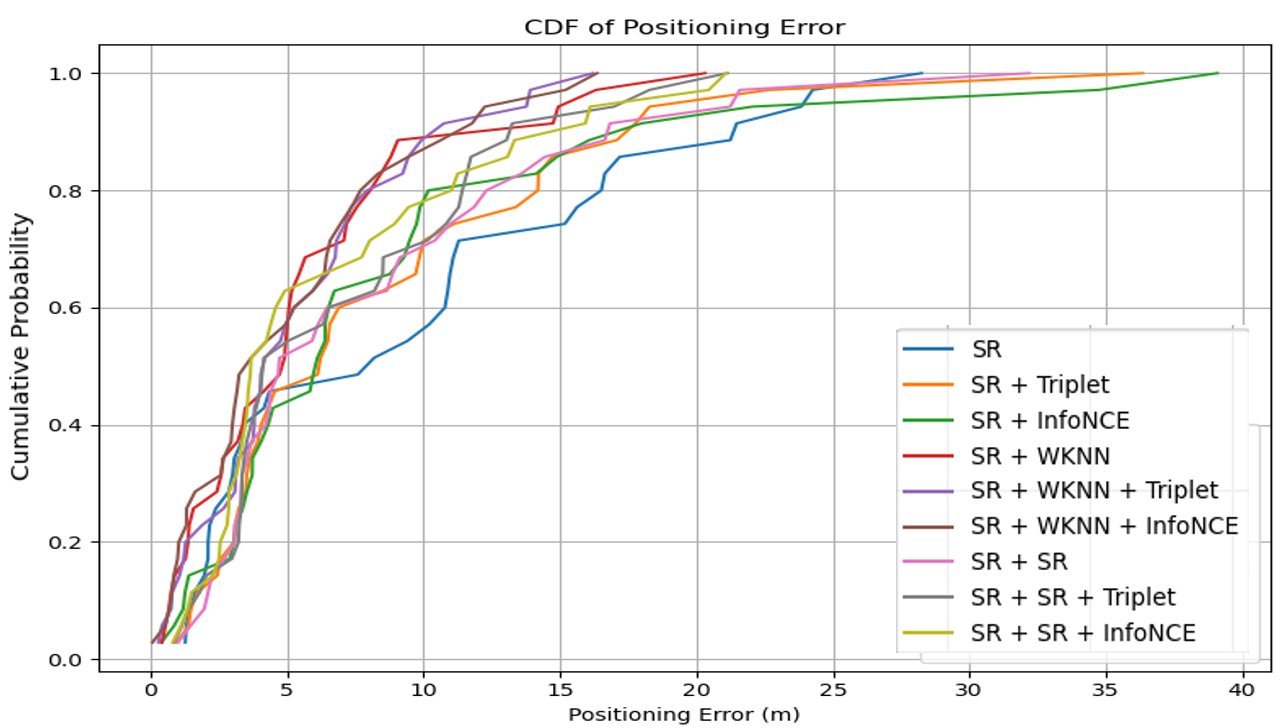
\includegraphics[width=0.7\columnwidth]{pics2/abba4.png}
\caption{CDF of localization error for SR-based methods}
\label{fig:cdf_srs}
\end{figure}
\begin{figure}[!t]
\centering
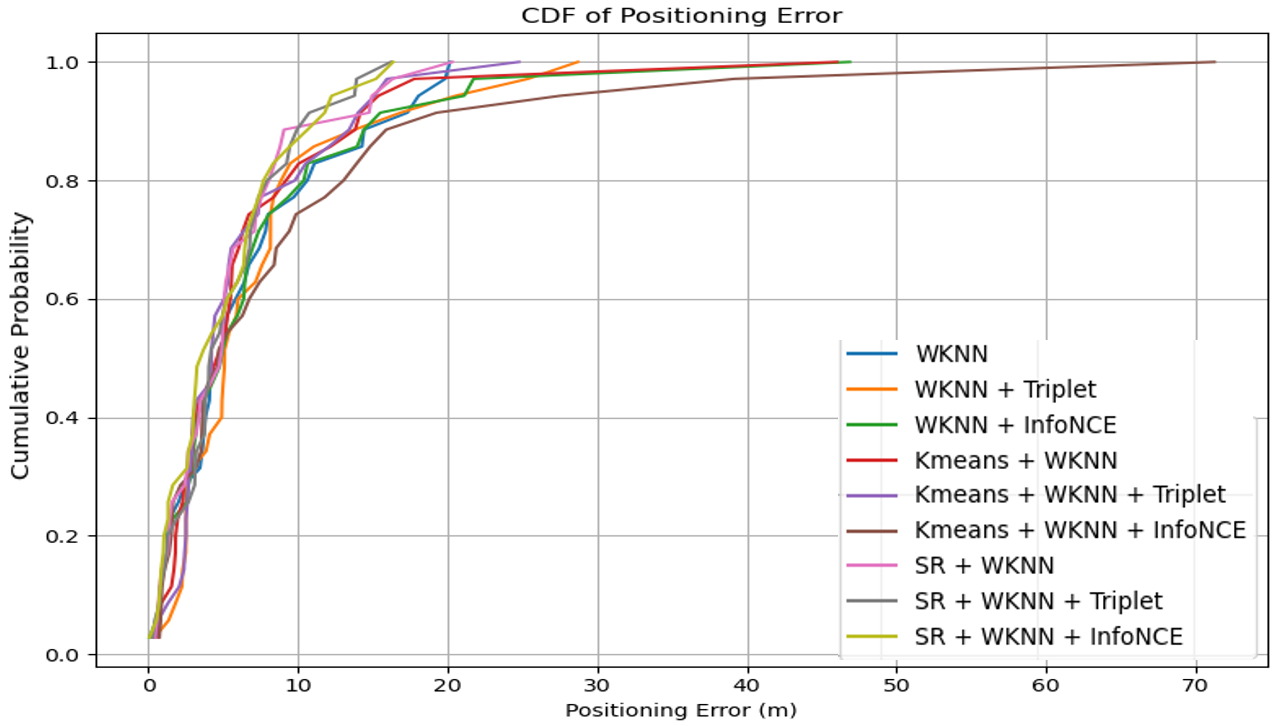
\includegraphics[width=0.7\columnwidth]{pics2/abba5.png}
\caption{CDF of localization error for WKNN-based methods}
\label{fig:cdf_wknns}
\end{figure}
% \subsubsection{Discussion}
\subsection{Results of Dynamic Localization}
\begin{table}[!t]
    \centering
    \caption{Mean Localization Errors for Dynamic Localization Using Kalman Filter with Various State Transition Models on the Custom Dataset.}
    \Huge
    \resizebox{\columnwidth}{!}{%
    \begin{tabular}{{ c | c | c | c | c }}
        \hline
        \textbf{Method} & \textbf{No-Kalman} & \textbf{Random Walk} & \textbf{Const. Vel} & \textbf{Const. Acc } \\
        \hline
        SR + WKNN & 2.30 & 2.18 & 0.98 & 0.97\\
        SR + WKNN + Triplet & \textbf{1.64} & \textbf{1.55} & \textbf{0.78} & \textbf{0.78} \\
        SR + WKNN + InfoNCE & 1.80 & 1.70 & 0.83 & 0.83\\
        \hline
    \end{tabular} %
    }
    \vspace{-10pt}
    \label{tab:dynamic_errors}
\end{table}

Table~\ref{tab:dynamic_errors} summarizes the results for dynamic localization with various state transition models on custom dataset. These models include random walk, constant velocity, and constant acceleration. Predicted locations using SR + WKNN method were used as measurements in all cases. 

The constant velocity (Const. Vel) and constant acceleration (Const. Acc) models lead to the lowest MLE across different methods (with a minimum of 0.78 m for SR + WKNN + Triplet). This suggests that these two models are more effective in predicting the state and improving localization accuracy and the random walk model may not be as effective as the these two models in this case.
In terms of the effect of contrastive representation learning, integrating triplet loss and InfoNCE loss into SR + WKNN decreases MLE compared to the baseline SR + WKNN method.
\subsection{Discussion} 
\label{sec:disc}
As observed in Table~\ref{tab:static_errors}, the K-Means + WKNN method does not perform well in the InfoNCE feature space, whereas the proposed SR + WKNN method achieves its best performance in this same space. 
This difference can be explained by the intrinsic characteristics of the embedding spaces learned by triplet loss and InfoNCE loss. 
While triplet loss is effective in forming well-separated local clusters by enforcing relative distance constraints among anchor, positive, and negative samples, it primarily focuses on local structure within individual triplets. 
This makes it particularly suitable for clustering-based approaches such as K-Means + WKNN, but it may fail to capture broader global relationships among samples.
In contrast, InfoNCE loss optimizes a contrastive objective over multiple negative samples, maximizing mutual information across samples. 
This results in embeddings that preserve more global and discriminative structures in the data.
In the SR + WKNN framework, accurate fine-grained localization relies heavily on distinguishing very close fingerprints in the feature space. 
Therefore, the richer and more globally consistent representations learned by InfoNCE provide better separability between nearby locations. 

Another important observation is the relative performance of the proposed SR + WKNN method across two learned feature spaces. 
As observed in Tables~\ref{tab:static_errors}, \ref{tab:benchmark_static_errors}, and \ref{tab:dynamic_errors}, SR + WKNN sometimes achieves better performance in the triplet space, while in other cases the InfoNCE space leads to lower localization errors. 
For example, in Table~\ref{tab:dynamic_errors}, the improvement achieved by SR + WKNN + InfoNCE  is less significant compared to SR + WKNN + Triplet. This happens similarly in Table~\ref{tab:benchmark_static_errors}  in terms of MLE for Geotec dataset.
One possible explanation for this behavior lies in the dependency of InfoNCE loss on dataset scale and diversity. 
As shown in Table~\ref{tab:benchmark_static_errors}, for the UJIIndoorLoc dataset, the InfoNCE space consistently achieves lower MLE values compared to the triplet space across all methods. 
In contrast, for smaller datasets such as the Geotec and Custom datasets, the difference between the two embedding spaces becomes less significant, and in some cases their performance is comparable.
This suggests that the effectiveness of each embedding space is influenced by dataset size and the variability of fingerprint distributions. 
InfoNCE is generally more effective in large-scale datasets where a rich set of negative samples is available, enabling stronger global discrimination, but in smaller-scale scenarios, triplet loss can still provide competitive performance.

According to Table~\ref{tab:static_errors} while the best performing method for custom dataset is SR + WKNN, for benchmark datasets (Table~\ref{tab:benchmark_static_errors}) 
the lowest errors belong to WKNN method.
It seems that with the increase in dataset size, the performance of SR-based methods decreases. Another limitation of the SR-based methods is their processing time which increases significantly compared to WKNN method, and this issue becomes more problematic in larger datasets with a considerably larger processing time. There are modern sparse representation approaches which aim to address this problem and reduce computation time, and their use can provide a potential solution.
\section{Conclusion }
This study introduces a novel dynamic indoor positioning framework based on Wi-Fi fingerprinting, which integrates contrastive representation learning, sparse representation, and Kalman filtering.
Experiments indicate that the learned spaces using contrastive learning effectively capture the spatial relationships within RSS data resulting in a significant improvement in localization.
Furthermore, the combination of SR with WKNN outperforms traditional methods on small datasets.
In the dynamic localization phase, Kalman filtering with a constant acceleration state-space model is incorporated to refine the position estimates over time. The results demonstrated that dynamic filtering significantly improved the positioning accuracy.
As future work, we will investigate the impact of negative sample selection strategies, collect a larger dataset, extend the framework to multi-floor positioning, and incorporate additional sensors.
\appendices
\section{Proof of Optimal Refinement}
\small
\textbf{\textit{Assumptions}:} 
\begin{enumerate}
    \item 
     The state transition and observation models are linear:  
	\begin{equation}  
	\mathbf{s}_t = \mathbf{A} \mathbf{s}_{t-1} + \mathbf{w}_t, \quad \mathbf{z}_t = \mathbf{H} \mathbf{s}_t + \mathbf{v}_t,   
	\end{equation}   
	with \(\mathbf{w}_t \sim \mathcal{N}(0, \mathbf{Q})\) and \(\mathbf{v}_t \sim \mathcal{N}(0, \mathbf{R})\).  
    \item 
    The static estimate \(\mathbf{\tilde c}_{x_t}\) serves as the noisy observation \(\mathbf{z}_t = \mathbf{\tilde c}_{x_t}\).  
\end{enumerate}

\textbf{\textit{Proof}:} 
 \begin{itemize}
     \item 
     \textbf{Step 1, Kalman Filter as Minimum Mean Squared Error (MMSE) Estimator:}  
	The Kalman filter recursively computes the posterior state estimate \(\hat{\mathbf{s}}_{t|t} = \mathbb{E}[\mathbf{s}_t | \mathbf{z}_{1:t}]\) and its error covariance \(\mathbf{P}_{t|t} = \mathbb{E}[(\mathbf{s}_t - \hat{\mathbf{s}}_{t|t})(\mathbf{s}_t - \hat{\mathbf{s}}_{t|t})^\top]\). By the Gauss-Markov theorem, it minimizes the MSE:  
	\begin{equation}   
	\mathbb{E}\left[ \| \mathbf{s}_t - \hat{\mathbf{s}}_{t|t} \|_2^2 \right] = \text{tr}(\mathbf{P}_{t|t}),  
	\end{equation} 
	where \(\text{tr}(\cdot)\) denotes the matrix trace.  
	\item 
    \textbf{Step 2, Static Localization as Unfiltered Observation:}  
	The static estimate \(\mathbf{\tilde c}_{x_t}\) corresponds to the observation \(\mathbf{z}_t = \mathbf{H} \mathbf{s}_t + \mathbf{v}_t\). Its MSE is:  
	\begin{equation}  
	\mathbb{E}\left[ \| \mathbf{c}_{x_t} - \mathbf{\tilde c}_{x_t} \|_2^2 \right] = \mathbb{E}\left[ \| \mathbf{H}\mathbf{s}_t - (\mathbf{H}\mathbf{s}_t + \mathbf{v}_t) \|_2^2 \right] = \text{tr}(\mathbf{R}).  
	\end{equation}   
    \item 
    \textbf{Step 3, Dynamic Localization MSE:} The dynamic estimate is \(\mathbf{\hat c}_{x_t} = \mathbf{H} \hat{\mathbf{s}}_{t|t}\). Its MSE is:
	\begin{equation} 
	\mathbb{E}\left[ \| \mathbf{c}_{x_t} - \mathbf{\hat c}_{x_t} \|_2^2 \right] = \text{tr}\left( \mathbf{H} \mathbf{P}_{t|t} \mathbf{H}^\top \right).  
	\end{equation} 
	 \item 
     \textbf{Step 4, Covariance Inequality:}  
	The Kalman filter ensures the posterior covariance satisfies:  
	\begin{equation}   
	\mathbf{P}_{t|t} \preceq \mathbf{P}_{t|t-1} \quad \text{(positive semi-definite ordering)},  
	\end{equation}  
	where \(\mathbf{P}_{t|t-1} = \mathbf{A} \mathbf{P}_{t-1|t-1} \mathbf{A}^\top + \mathbf{Q}\) is the prior covariance. Since \(\mathbf{R}\) represents the static localization noise, we have:  
	\begin{equation}  
	\mathbf{H} \mathbf{P}_{t|t} \mathbf{H}^\top \preceq \mathbf{R}.  
	\end{equation}   
	Taking the trace on both sides:  
	\begin{equation} 
	\text{tr}\left( \mathbf{H} \mathbf{P}_{t|t} \mathbf{H}^\top \right) \leq \text{tr}(\mathbf{R}).  
	\end{equation}   
 \end{itemize}
\textbf{Conclusion}:  
\begin{equation}  
\mathbb{E}\left[ \| \mathbf{c}_{x_t} - \mathbf{\hat c}_{x_t} \|_2^2 \right] \leq \mathbb{E}\left[ \| \mathbf{c}_{x_t} - \mathbf{\tilde c}_{x_t} \|_2^2 \right].  
\end{equation}  
Thus, the Kalman-filtered dynamic estimate achieves equal or lower MSE than the static estimate.  
\(\blacksquare\) 
\bibliographystyle{IEEEtran} 
\bibliography{references}

\end{document}
